\chapter{尤度比を使ったモデルとデータの比較}
モデル$M$において得られるデータ元に、母数を最尤推定する。新たに作られた最尤モデル上での尤度と元のモデル$M$での尤度の比がある分布に従うことがわかっている。
このことを利用して、もともモデル$M$でデータを予測してもいいのかを考察する。

前の章で統計検定をモデル鳥によって説明した。あるモデル鳥が生んだ標本卵に関する統計量のばらつきの特徴と、研究者が持ってきたデータ卵を比較し、そのモデル鳥が産んだと判定していいのかを考える方法と説明した。
ここでも、どのモデルが生んだ標本卵に関わる予測なのかを考えなくてはならない。
あるフルモデルにおける予想分布をまずは考察する。

\section{概要}

\begin{defi}
    母数の数が異なる統計モデル間の尤度の比を次のように定義する。
    \begin{equation*}
        Dev(D,M_1,M_2) = -2\log\frac{M_1におけるDの尤度}{M_2におけるDの尤度}
    \end{equation*}
    ここで、$M_1$は、$M(\theta_1,\theta_2)$,$M_2$は$M((\theta_{1'},\theta_2))$であり、$\theta_1$と$\theta_2$のベクトルの要素数の和は、$\theta_{1'},\theta_2$のベクトルの要素数の和に等しい。$D$は標本とする。

\end{defi}

$M_1$における標本$D$から、最尤モデル$M_1(\hat{\theta_1})$を構築したとき、$Dev(D,M_1,M_1(\hat{\theta_1}))$は、
\begin{equation*}
    Dev(D,M_1,M_1(\hat{\theta_1})) \sim \chi^2_{p}
\end{equation*}
であることがわかる。ここで、$p$は、$\theta_1$の要素数。
例えば、正規モデル$M(170,5.8^2)$から標本$D$を生成する。その$\mu$に対する最尤モデル$M(\hat{\mu})$は、次のようになる。
\begin{equation*}
    Dev(D,M(170,5.8),M(\hat{\mu})) \sim \chi^2_1
\end{equation*}
データ由来の母数の個数が$1$なので、自由度$1$の$\chi^2$分布に従う。

あるデータ$D'$に対して、最尤推定を行なったモデル$\hat{M}$について、次のことがわかる。
\begin{equation*}
    Dev(D,\hat{M},\hat{\hat{M}}) = -2\log\frac{\hat{M}におけるDの尤度}{\hat{\hat{M}}におけるDの尤度} \sim \chi^2_{p}
\end{equation*}
ここで$D$は、$\hat{M}$の標本であり、$\hat{\hat{M}}$は、標本$D$を使って$\hat{M}$のいくつかの母数の最尤推定を行なったモデル、$p$は$\hat{\hat{M}}$において最尤推定を行なった母数の個数。

\subsection{データと当てはめモデル$\hat{M}$の比較}
データ$D$を当てはめていないモデル$M$に対して、$D$を予測できるかを確かめる。
パラメータの個数が少ないモデル$M'$についての尤度比は次で計算できる。
\begin{equation*}
    Dev(D,M,M')
\end{equation*}
$M$によって、$D$について十分な予測ができるならば、パラメータを任意の個数減らしたモデル$M'$との尤度比は、$Dev(D,M,M')$が自由度は元のパラメータ数-自由度+1となる$\chi^2$分布に従う。
このことから、$Dev(D,M,M')$が比較的小さな値であれば($p$値は比較的大きくなっている)、モデル$M$によって予測可能であることの根拠の一つになりうる。


\subsection{データと当てはめモデル$\hat{M}$の比較}
当てはめたモデル$\hat{M}$とデータの比較。
次を計算する。$D'$を観測データとする。
\begin{equation*}
    Dev(D',\hat{M},\hat{\hat{M}}) 
\end{equation*}
ここで、$M$の標本$D'$の最尤推定モデルを$\hat{M}$とし、$\hat{\hat{M}}$は$\hat{M}$の$p$個の母数に対して最尤推定を行なったモデルである。
$Dev(D,\hat{M},\hat{\hat{M}}) $の分布($\chi^2_p$)の中で、$Dev(D',\hat{M},\hat{\hat{M}}) $が珍しい値を取っていたなら、
$\hat{M}$から考えられる尤度比の変動の中では、比較的大きな変動が起きていることが示唆される。
このことから、$\hat{M}$で標本を予想しない方が良いのではないだろうかと判断する。

注意しなければいけないのは、$\hat{\hat{M}}$の方が良いとは言えてないことである。
当てはまりの良さは、尤度の大小関係を見れば良い\footnote{次は何かがおかしい「尤度の大小関係が有意であることを確かめるのが尤度比検定である。」。}。%有意かどうかとはどういう意味かがわからない。$\hat{M}$の尤度比の変動では予測できないという意味であれば理解できる。さまざまな前提で検定が使われているので、解釈が一致しない。}。

\if 0
この性質を利用して、母数の数の異なるモデルに対して、最尤推定をそれぞれ行い、モデルを構成する。
ある統計モデル$M_1$とし、$M_1$の中でいくつかの母数を固定したモデル$M_2$とする。
$M_1$からサンプリングした標本とその最尤モデル$M_{1'}$は尤度の比が$\chi^2$に従う。
同様に、その標本に対する最優モデル$M_{2'}$とすれば、$M_1$と$M_{2'}$の尤度比も$\chi^2$分布に従う。

ここで、母集団から無作為抽出した標本$D$とする。
$D$の最尤モデルを$M_{1''}$、$M_{2''}$とする。
これらモデル上での尤度の比を計算し、$\chi^2$においてどの程度の珍しさなのかを調べる。


そのモデルでのならば、どの程度の珍しさなのかを計算する。
尤度比が大きくなれば、$\chi^2$において珍しい値になり、$p$値が小さくなる。
言い換えれば、あるモデルで予想される尤度の比と比べて、データから導かれた尤度比が大きな変動かが計算できる。
\fi

\begin{SMbox}{尤度比検定で$p<0.05$だったので$M_1$より$M_2$がより適合的だ}
    尤度比検定で$p<0.05$だったので$M_1$より$M_2$がより適合的だという判断はしないほうが良い。
    尤度比検定において$p$値が小さいということは、
    $M_1$における尤度比の予測値の中で、比較的大きな尤度の変化が実験データでは生じていることを示したことになる。
    これは、$M_1$の中での変動と比較しているだけである。
    相対的に$M_2$の方がより適合的であることを示唆していない。
    
    より適合的であることを示す量は、尤度である。
    対数尤度が小さい方がデータに対して適合しているという判断ができる。
\end{SMbox}



\if 0
\paragraph{尤度比}
データを指数分布から生成し、モデルを正規モデル$M$とする。
二つの母数についての最尤モデルと、平均
このとき、何度もデータを指数分布から生成し、尤度比を計算したとき、その尤度比は$\chi^2$に従うか?
%無作為抽出して得た標本に対して、あるモデルのその標本に対する最尤モデルを$M(\theta_1,\theta_2,\theta_3)$とする。
\fi

\section{尤度比検定}
母数の個数が$k$個のモデル$M(\theta)$とする($\theta$は$k$次元ベクトル)。
モデル$M(\theta)$からサンプリングしたサンプルサイズ$n$の標本$x=(x_1,x_2,\cdots,x_n)$を得たとする。
この標本$X$から$\theta$のうち$r$個の母数に関する最尤推定量を$\bar{\theta}$得たとする。
$\bar{\theta}$のうち$k-r$個はモデル由来の母数であり、$r$個は標本から推定した母数である。
このことから、$\bar{\theta}$は自由度$r$の母数のベクトルと言う。

もとのモデル$M(\theta)$における標本$X$に対する尤度は、$L(\theta,x)$とする。
また、最尤モデル$M(\bar{\theta})$での尤度は、$L(\bar{\theta},x)$とする。
このとき、これら尤度の比がカイ二乗分布分布に従うことがわかっている\footnote{ただしいくらかの条件がある}。
つまり、
\begin{equation*}
    -2\log\lambda(X)\sim \chi^2_{k-r}
\end{equation*}
ただし、
\begin{equation*}
    \lambda(X) = \frac{L(\theta,x)}{L(\bar{\theta},x)} 
\end{equation*}
である。


\begin{SMbox}{滅多に観察されない逸脱度}
\begin{quote}
    有意確率が小さければ(通常は$5\%$以下)\footnote{おそらく$p$値が小さければ}、2つのモデルの「逸脱度の差」は滅多に観察されないほど大きな値であると判断する。
\end{quote}
    これは本書とは異なる方針の科学における指針である\footnote{
        この話は後でもう一度考えて見た方がいい気がする。
        できないはずであるが、できるとする論文が多い。なぜなんだろうTODO。
    }。

    本書では、ある統計モデルが予測した統計量と比較して大きな統計量が得られたからといって、現実的に滅多に観察されないとは解釈しない。

    本書が扱いたい科学において、
    一般化線型モデルを使えば、現実での起こりやすさが検証できるということはおそらくない。
    %https://www.jstage.jst.go.jp/article/weed/55/4/55_4_275/_pdf
    %特集 統計解析(再?)入門 R を用いた一般化線形モデル(仮説検定編): 割合データを例
\begin{quote}
    2つのモデルの「逸脱度の差」が大きいことから、すなわち、要因を覗くことでモデルの当てはまりが十分に悪くなることから、その要因は有意な要因であると判断する。
\end{quote}
    これも本書とは異なる分野を研究しているのだと思われる。

    尤度比の差の統計量を実データの尤度比の差と比べてわかるのは、フルモデルで予測または当てはめしない方が良さそうということである。
    より当てはまりのモデルかどうかは尤度比を比べればよい。
\end{SMbox}

\section{正規モデルにおける尤度比検定}

$\sigma^2_0$を設定した正規モデル$M(\mu_0;\sigma^2_0)$について考察する。
この正規モデルからサンプリングを行なった標本$X$とする。
標本から得た最尤正規モデルを$M(\bar{x};\sigma^2_0)$とする。
それぞれのモデル内での標本$X$の尤度を$L(\mu_0,X),L(\bar{x},X)$とする。
具体的な数式は、
\begin{align}
    L(\mu_0,X)=\frac{1}{\sqrt{2\pi\sigma^2}}\exp(-\frac{\sum(x_i-\mu_0)}{2\sigma^2})\\
    L(\bar{X},X)=\frac{1}{\sqrt{2\pi\sigma^2}}\exp(-\frac{\sum(x_i-\bar{X})}{2\sigma^2})\\
\end{align}
これらから$\lambda(X)$を計算すると、
\begin{align}
    -2\log\lambda(X) &= -2(-\frac{n}{2\sigma^2_0}(\bar{x}-\mu_0)^2) \\
    &= \frac{n}{\sigma^2_0}(\bar{x}-\mu_0)^2 \sim \chi^2_1 \\
\end{align}
である。

\subsubsection{数値実験}
モデルと同じ確率密度関数からサンプリングを行い、尤度比検定を行なってみる。

数値実験を行なってみる。具体的に、正規分布$N(170,5.8^2)$からサンプリングした標本1000個を集める。
標本から平均値を求め、これを最尤推定量とする(xbar)。
この最尤モデル$M(\mu;\sigma^2=5.8^2) $における標本の尤度を計算する(loglike2)。
同様に、モデル$M(170;\sigma^2=5.8^2)$における標本の尤度を計算する(loglike)。
以上から尤度比を計算し、それが$\chi^2_1$分布と一致することを確かめる。
以下がコードである。

\begin{lstlisting}
norm_ = norm(170,5.8)
data_ = norm.rvs(170,5.8,size=(1000,10))
xbar = np.average(data_,axis=1)
loglike_ = np.prod(norm_.pdf(data_),axis=1)
#loglike2_ = np.prod(norm(xbar,5.8).pdf(data_),axis=0)
#print(np.prod(norm(xbar,5.8).pdf(data_),axis=1),xbar)

loglike2_ = []
for item in data_:
    #print(item.shape)
    a = norm(np.average(item),5.8).pdf(item)
    loglike2_.append(np.prod(a))

y = -2*np.log(loglike_/loglike2_)
x = sorted(y)
y_ = np.arange(len(y))/len(x)
plt.plot(x,y_)
plt.plot(x,chi2.cdf(x,df=1))
plt.show()

\end{lstlisting}

$N(170,5.8^2)$と$N(175,5.8^2)$と言う2種類の密度関数からサンプリングを行いそれぞれ結果を図\ref{fig:loglikelihood_test_simulation_norm}(a)および(b)に示す。
図\ref{fig:loglikelihood_test_simulation_norm}(a)は、モデルとデータの分布が一致していることから、累積分布が$\chi^2_1$の累積分布にかなり近いことがわかる。
図\ref{fig:loglikelihood_test_simulation_norm}(b)は、モデルとデータが一致していない状況での結果を示している。尤度比の多くが右に移動しており、標本の多くが$\chi^2_1$において珍しいと判定されやすくなっている。


\begin{figure}
    \begin{center}
        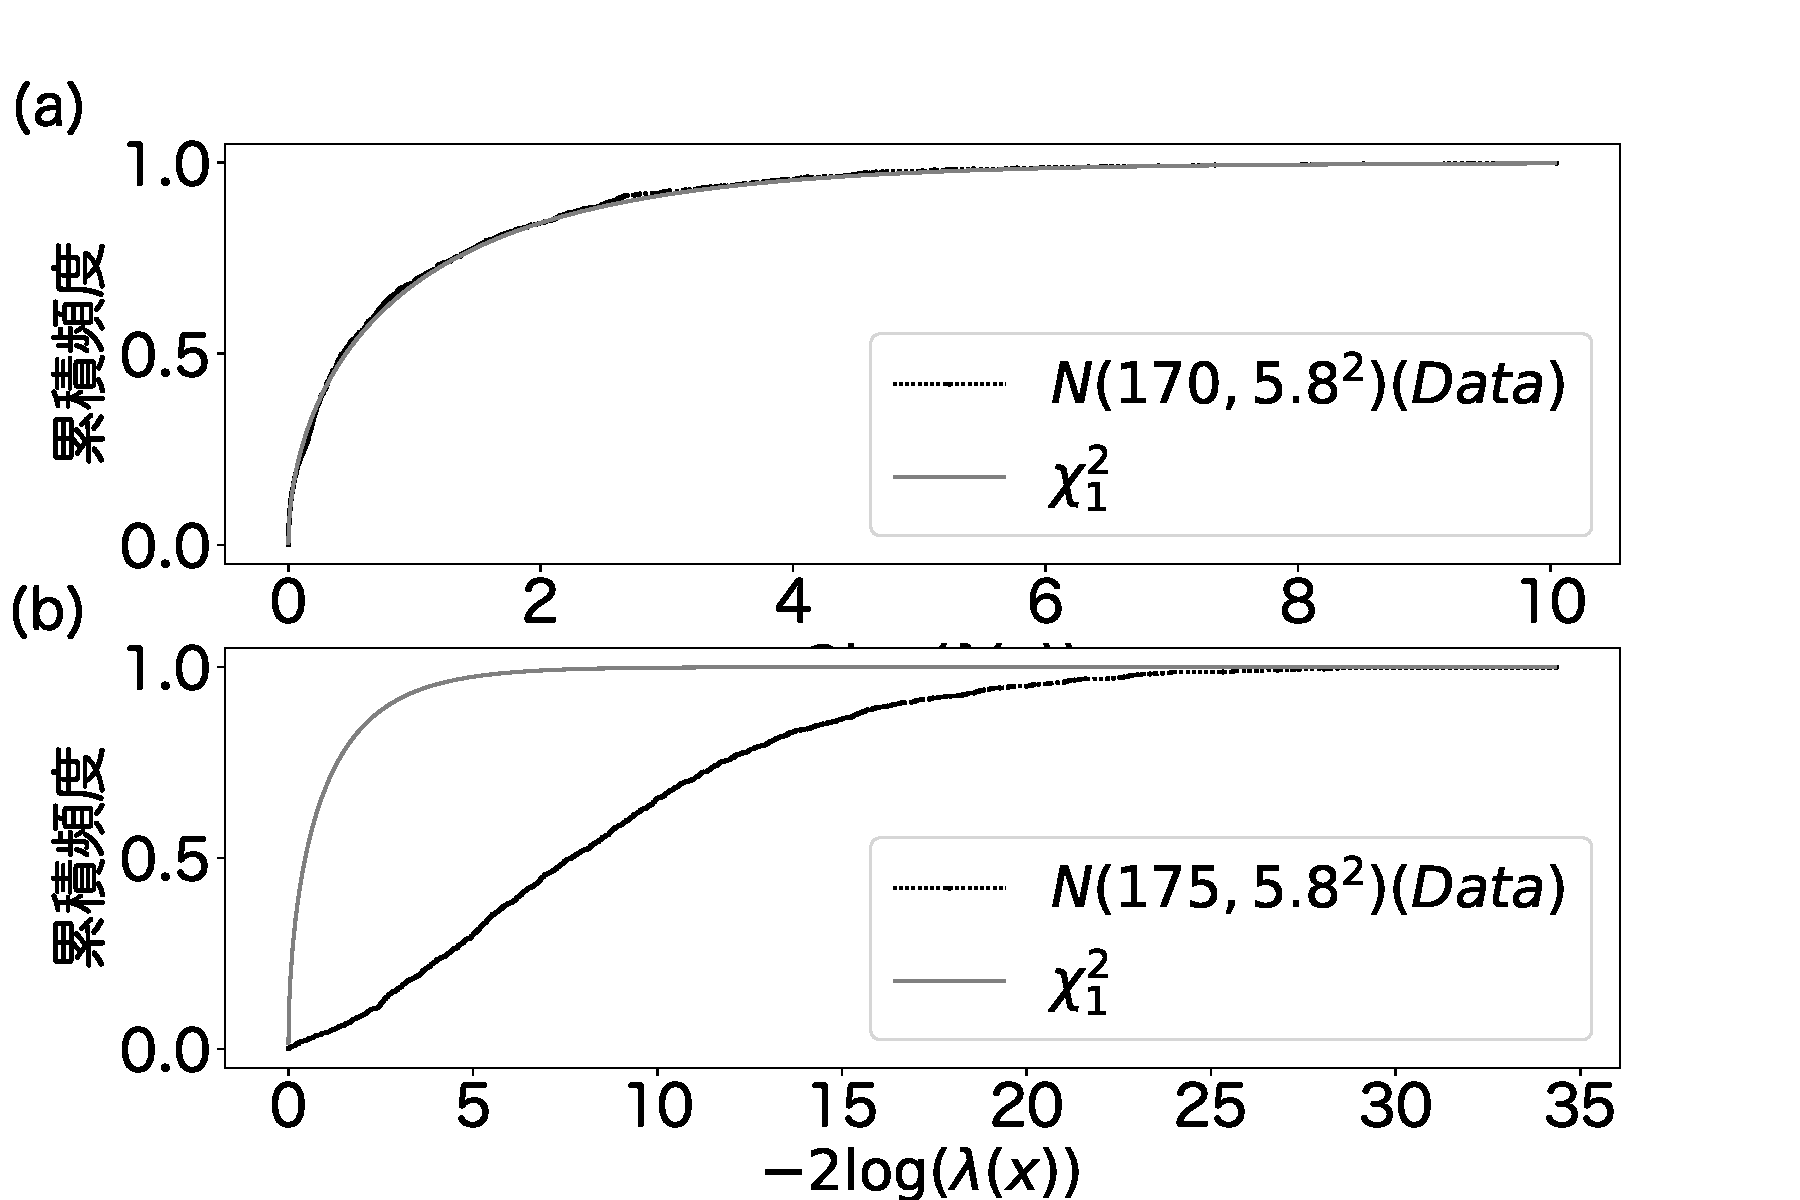
\includegraphics[width=15cm]{./image/04_/loglikeli_norm_test.pdf}
        \caption{対数尤度比の累積頻度。モデルは正規モデル$M(170;\sigma^2=5.8^2)$。(a)標本を$N(170,5.8^2)$からサンプリングした結果。(b)標本を$N(175,5.8^2)$からサンプリングした標本。}
        \label{fig:loglikelihood_test_simulation_norm}

      \end{center}
    \end{figure}

\subsection{データとモデルの乖離を検証する}
モデル上において、その標本を元にした最尤モデルにおける尤度比が$\chi^2_1$に従うことを示した。このことを元に、データをモデルによって予測可能かを調べる。手順は、
\begin{enumerate}
    \item 標本を$x$とする。
    \item モデル$M$における最尤推定量を計算する。
    \item モデル$M$および最尤モデル$M_{MLE}$における標本$x$に対する尤度を計算する
    \item 尤度比および$-2\log\lambda(x)$を計算し、$\chi^2_1$において珍しい値なのかを検証する。
\end{enumerate}
実際に、正規モデルにおいてこの手順をなぞってみる。
$M(\mu;\sigma^2)$における最尤モデルは、$M(\bar{x};\sigma^2)$である。
それぞれのモデルにおける尤度を計算し、$-2\log\lambda{x}$を計算すればよい。

\section{複雑なモデルでの尤度比検定}
次のモデル$M(\beta_1,\beta_2)$を考える。
\begin{enumerate}
    \item $x_i$は定数。
    \item $y_i$は以下に示す分布$p(y_i;\lambda_i)$に従う。
    \item $\lambda_i = \exp(\beta_1+\beta_2 x_i)$
    \item $y_i \sim p(y_i;\lambda_i) = \frac{\lambda_i^{y_i}\exp(-\lambda_i)}{y_i!}$
\end{enumerate}
無作為抽出した標本$x$における2つの最尤モデルを考える。
最初のモデルは、$\beta_2=0$とした上で、$\beta_2$に関する最尤推定を行なったモデル$M_1=M(\hat{\beta_1},\beta_2=0)$である。
このモデルでは、$x_i$に応じて、$\lambda_i$が変化しないので、$\lambda$が常に一定のモデルになる。言い換えれば、$y$が母数$\lambda=\exp(\beta_1)$のポアソン分布となるモデルである。
次のモデルは、$\beta_1,\beta_2$の両方について最尤推定を行なったモデル$M_2=M(\hat{\hat{\beta_1}},\hat{\hat{\beta_2}})$である。
このモデルにおいて、$(x_i,y_i)$はペアになっており、$x_i$に応じて$y_i$が揺らぎを持って決まる。

ここで、$M_1$における尤度比が$\chi_1^2$に従うことを確かめる。手順は以下の通りである。
\begin{enumerate}
    \item $M_1$においてサンプリングを行い、$(x_i,y_i)$からなる標本$X$を得る。$x_i$は、既存の標本$x$のものを使う。$(x_i,y_i)$に関してバラバラになった標本が得られる。
    \item $M_1$における標本$X$の尤度$L_1$を計算する。
    \item $M_2$における標本$X$の尤度$L_2$を計算する。
    \item $-2\log\frac{L_1}{L_2}$を計算する。以上を繰り返す。
\end{enumerate}
以上を行うと、$\chi^2_1$に従うことがわかる。図\ref{fig:loglikelihood_test_simulation_poisson}a,bに結果を載せている。
コードを書いておく。
\begin{lstlisting}
df  = pd.read_csv("https://raw.githubusercontent.com/tushuhei/statisticalDataModeling/master/data3a.csv")

def get_dd(d):
    d['y_rnd'] = np.random.poisson(np.mean(d.y),len(d.y))
    model1 = smf.glm(formula='y_rnd~1',data=d,
    family=sm.families.Poisson())
    model2 = smf.glm(formula = 'y_rnd~x',data=d,family=sm.families.Poisson())
    #print(fit1.summary())
    fit1 = model1.fit()
    fit2 = model2.fit()
    return fit1.deviance - fit2.deviance

l = []
for i in range(1000):
    l.append(get_dd(df))


x = sorted(l)
y = np.arange(len(l))/len(l)
plt.plot(x,y)
plt.plot(x, chi2.cdf(x,df = 1))
plt.show()
\end{lstlisting}


\begin{figure}
    \begin{center}
        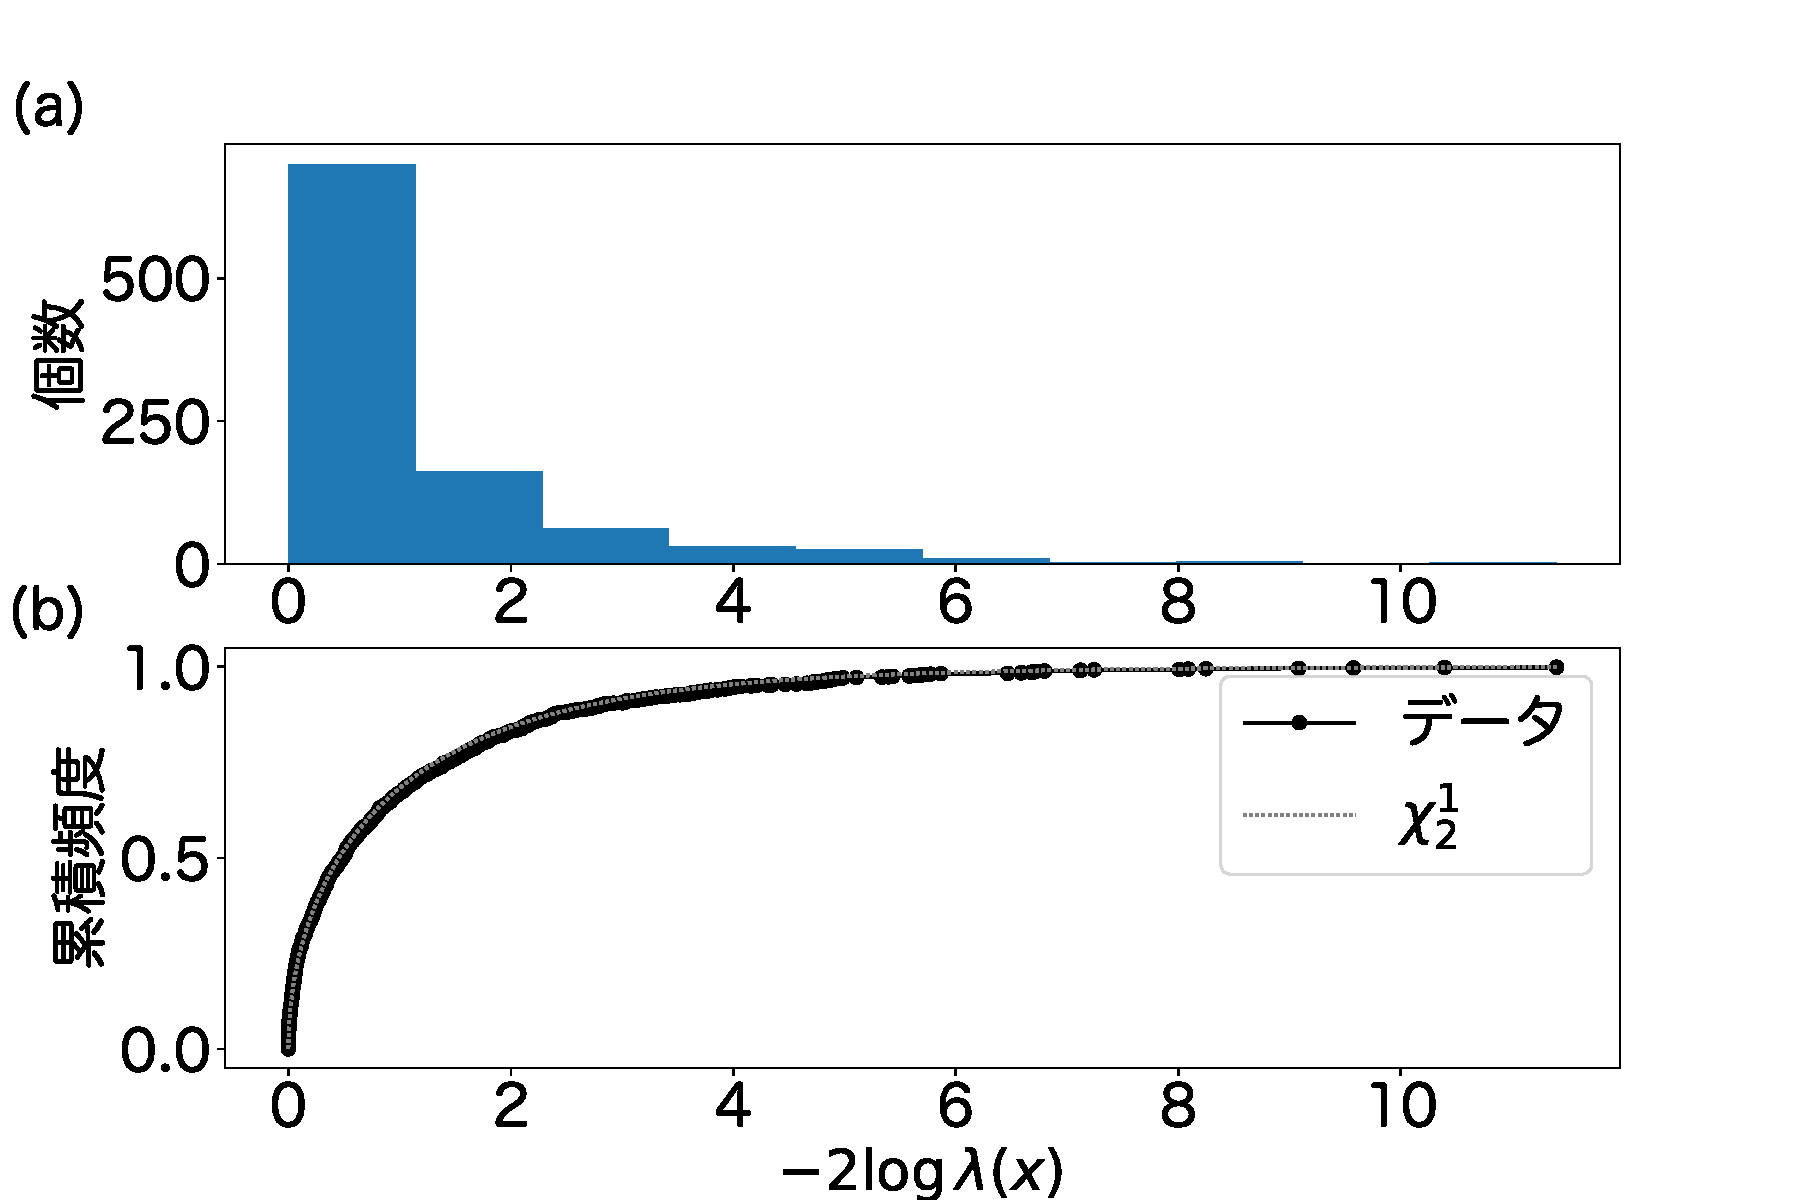
\includegraphics[width=15cm]{./image/04_/loglikeli_poisson_model_test.pdf}
        \caption{$M_1$における対数尤度比の累積頻度。(a)ヒストグラム(b)累積分布}
        \label{fig:loglikelihood_test_simulation_poisson}
    \end{center}
\end{figure}


データと、最尤モデル$M_1$との比較は同様に、
\begin{enumerate}
    \item 標本$x$の尤度$L_1$を$M_1$上で計算する。
    \item 標本$x$の尤度$L_2$を$M_2$上で計算する。
    \item $-2\log\frac{L_1}{L_2}$を計算する。
\end{enumerate}
最尤モデル$M_1$においてデータ$x$が予測できないなら、$-2\log\frac{L_1}{L_2}$が大きな値を取る。

最尤モデル$M_1$からサンプリングされた標本の尤度と、最尤モデル$M_2$での尤度を比較すると、$\chi^2_1$に従う。
なぜならば、ここにおける最尤モデル$M_2$のパラメータ$\beta_2$はほとんど0と変わりなく、小さな値をとるので、$M_1$と違いが少ない。
標本が$M_1$からサンプリングされていないなら、モデル$2$での最尤推定の結果、
$\beta_2$も$0$から離れてしまい、尤度比も大きくなるはずである。
$M_1$で標本$x$を予測しない方がよくないことを示す証拠の一つになる。
ただし、$M_2$が良い予測モデルであるのかは不明である。


$M_1$からサンプリングした標本で、$M_1$および$M_2$を推定したモデルの尤度比は$\chi^2_1$に従う。
実際の標本を元に、$M_1,M_2$を推定し、そのモデルの尤度比は、$M_1$による予測ができるならば、$\chi^2_1$程度だと考えられる。
実際にこの例では、尤度比が大きくなり、$\chi^2_1$においては珍しい値になったので、
$M_1$により予測しない方が良さそうと言う根拠の一つになりうる。
$M_2$の$\hat\hat\beta_2$のパラメータがどうなっているかなども気にした方が良さそう。



\begin{SMbox}{帰無仮説の取り方}
    \if 0
    \begin{theorem}
        $M_a$を$M_b$のネストされたモデルとする($M_b$の方が$M_a$よりもパラメータが多い)。このとき、$M_a$からサンプリングした標本$X$について、
        \begin{equation*}
            -2\log\frac{M_aにおけるXの尤度}{M_bにおけるXの最尤推定量}
        \end{equation*}
        は、ある自由度を持つカイ二乗分布に従う。
    \end{theorem}
\fi

    通常の尤度比検定は、次の通りである。
    \begin{theo}
        帰無仮説:$M_a=M(\alpha)$\\
        対立仮説:$M_b=M(\alpha,\beta\neq 0)$\\
        とする。このとき次が自由度1のカイ二乗分布に従う。
        \begin{equation*}
            -2\log\frac{帰無仮説における尤度}{サンプルXを元にした最優M(\alpha,\beta)での尤度}
        \end{equation*}
    \end{theo}

    「データ解析のための統計モデリング入門」では定理として示されてはいないが、恣意的にまとめてみると次のことが成立していると考えられている。
    \begin{theo}
        帰無仮説:$M_a=M(\alpha)$\\
        対立仮説:$M_b=M(\alpha,\beta\neq 0)$\\
        とする。このとき、次が自由度1のカイ二乗分布に従う。
        \begin{equation*}
            -2\log\frac{帰無仮説における尤度}{M(\alpha,\beta\neq 0)の最尤モデルにおける尤度}
        \end{equation*}
    \end{theo}
    尤度比が、頻度論統計学で紹介されるものとは異なっている。これが成立するのかは私にはわからないので、本書では採用していない。

    また、本書と異なる点は、対立仮説を採択している点である。
    \begin{quote}
        So we can state that 対立仮説 can be accepted.\footnote{\url{https://kuboweb.github.io/-kubo/stat/2019/Ees/d/kubostat2019d.pdf}}
    \end{quote}

    本書においては、尤度比検定ではモデルとの乖離を調べれるという方針なので、モデルとデータを比較していないモデルを採択することはありえない。    
\end{SMbox}



\section{One-way ANOVA}
次の仮定をもとに統計モデル$M_A=M(\mu_1,\mu_2,\cdots,\mu_n)$を構築する。
\begin{enumerate}
    \item $\mu_i (i=0,1,2,\cdots,n)$
    \item $x_{ik} \sim N(\mu_i,\sigma^2)$
\end{enumerate}
この統計モデルの$\mu_1=\mu_2=\cdots=\mu_n$としたときの最尤推定量を計算する。
サンプリングされた標本$x = x_{ik} (k=0,\cdots,n_i)$とすると、このモデルの尤度は次のようになる。
\begin{equation*}
    L(\mu;x) = \prod_{i=0,1,2,\cdots,n,k=0,2,\cdots,m_i}\frac{1}{\sqrt{2\pi\sigma^2}}\exp(-\frac{(x_{ik}-\mu_i)}{2\sigma^2})
\end{equation*}
最尤推定量は次のようになる。
\begin{equation*}
    \bar{\mu_i} = \frac{1}{n_i}\sum_{j=0}^{n_i} x_i = \bar{x_i},\\
    \bar{\sigma}^2 = \frac{1}{\sum_{i}^k n_i} \sum_{i=0}^n \sum_{j=0}^{n_i} (x_{ij}-\bar{x_i})^2
\end{equation*}
である。

このモデルについて母数制限を制限したモデルを$M_N=M(\mu;\sigma^2)$がある。
$M_N$は明らかに$M_A$のネストされたモデルである。
$M_s$から得られたサンプル$x$についてその最尤推定量は次のようになる。
\begin{equation*}
    \bar{\mu}_{\rm{ML}} = \frac{1}{\sum_{i=0}^n m_i} \sum_{i=0}^n\sum_{k=0}^{m_i} x_{ik}, \\
    \bar{\sigma^2}_{\rm{ML}} =  \frac{1}{\sum_{i=0}^n m_i} \sum_{i=0}^n \sum_{k=0}^{m_i}(x_{ik} -\mu)^2
\end{equation*}
以上をもとに尤度比を計算する。
\begin{equation*}
    -2\log \lambda(x) = \frac{L(\mu;\bar{\sigma}^2)}{L(\mu_1,\mu_2,\cdots,\mu_n,\bar{\sigma}^2_{ML})}
\end{equation*}

$M_N$において、このモデルの上位の$M(\mu_1,mu_2,\cdots,\mu_n)$の最尤推定モデルと、$M_N$の尤度比がカイ二乗分布に従う。
検定統計量は以下の通り。
\begin{equation*}
    F = \frac{\sum_i^k \frac{n_i (\bar{x}_i-\bar{x})^2}{k-1}}{ \sum_{i=0}^k\sum_{j=0}^{n_i}\frac{ (x_{ij}-\bar{x}_i)^2 }{n-k}}
\end{equation*}
データ由来の母数の個数から1を引いた数が自由度になる。
つまり、
$-2\log\lambda(x)\sim \chi^2_{k-1}$である。

モデル$M_N$における統計的性質であることに注意。
以上のことから、1つの平均値を設定したモデルとデータが乖離していることを調べることができる。


\begin{SMbox}{少なくとも一つは母数が違う}
    1-way ANOVAを使い、$p<\alpha$を得たならば、少なくとも一つは母数が違う郡が入っている。言い換えれば、帰無仮説が棄却され、対立仮説を採択している。    
    有意差検定では、対立仮説を採択することはないと説明している教科書でも、ANOVAでは対立仮説を採択していることがある。
    
    ここで得られる主張は、$M_N$モデルとデータが乖離しているかもしれないである。
    異なる母数で推測した方が良いという結論を得るには、検定以外の方法で、データを解析することが必要である。
\end{SMbox}

\subsection{数値計算}
統計的性質が現れることを数値計算により確かめてみる。
\begin{lstlisting}
mu = 170
sigma=5.8
n=10
sampleN = 200

norm_ = norm(mu,sigma)
l=[]
for i in range(10000):
    sample = norm_.rvs(size=(n,sampleN))

    ave_ = np.average(sample)
    sigma_ = np.std(sample) 
    #sigma_,ave_
    ave_s = np.average(sample,axis=1)
    sigma_s = np.std(sample,axis=1)
    ave_s.shape,sigma_s.shape

    lam = np.sum( (sample - ave_)**2)/np.sum( (sample.T - ave_s)**2)
    l.append((sampleN*n)*np.log(lam))

x = np.sort(l)
y = np.arange(len(l))/len(l)
plt.plot(x,y)
plt.plot(x ,chi2.cdf(x,df = n-1))
plt.show()
\end{lstlisting}